\graphicspath{{results/fig/}}

\chapter{Results}
\label{chap:results}
An incremental approach to testing was done for this project. Each software component was tested individually. This section will report on the results of the incremental testing as well as the results of the entire system. Lastly the entire system will be used to calculate the mean square flux noise figure of an actual SQUID design with measured mean square flux noise values.

\section{The noise extraction module}
The accuracy of this module is tested by comparing its output to a numerical solution for the given geometry. This module is tested without mesh optimisation. It is tested before the mesh optimisation module because the test setup for the mesh optimisation module requires the use of the noise extraction module.
\subsection{Test setup}

Equation \ref{eq:MSFNfinal} describes the analytical solution for a thin wire loop. The assumption made in the derivation of this equation is that $R >> D$. The test is performed was a parameter sweep from $R = \si{8}{\mu m}$ and $D = \si{5}{\mu m}$ to $R = \si{45}{\mu m}$ and $D = \si{0.4}{\mu m}$ as shown figure \ref{fig:meshedTorus}. The parameter sweep was automated using a python script.

\begin{figure}[h]
    \centering
    \begin{subfigure}[b]{0.45\textwidth}
        \centering
        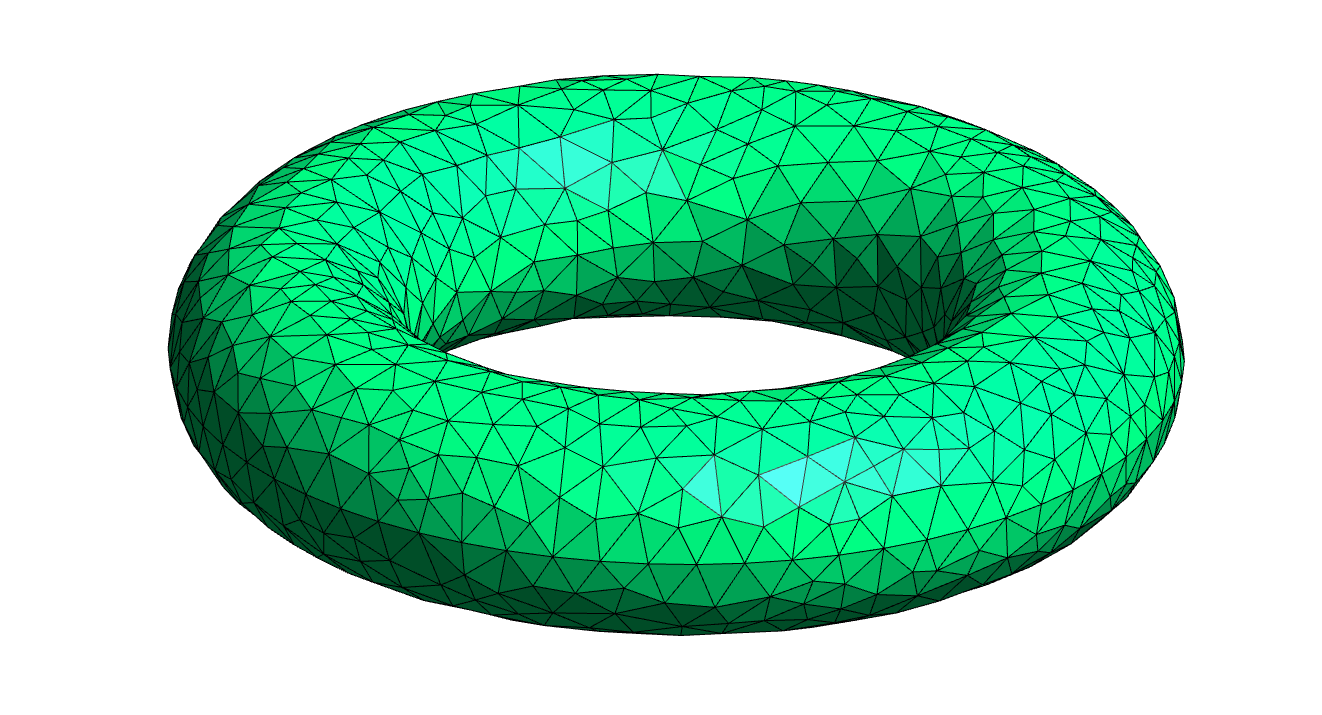
\includegraphics[width=0.5\textwidth]{torusThick}
        \caption{The meshed torus with the smallest loop radius and largest wire diameter}
    \end{subfigure}
    \hfill
    \begin{subfigure}[b]{0.45\textwidth}
        \centering
        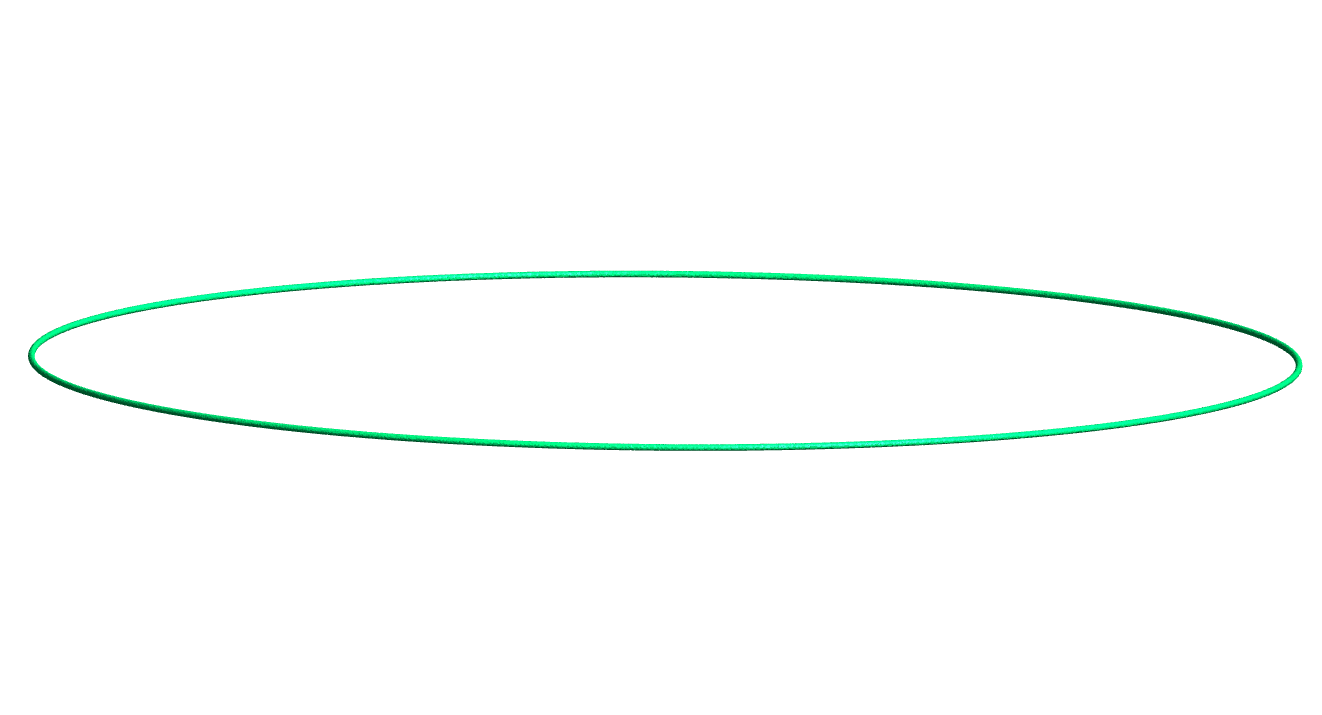
\includegraphics[width=0.5\textwidth]{torusThin}
        \caption{The meshed torus with the largest loop radius and smallest wire diameter}
    \end{subfigure}
    \caption{A figure showing the two extremes of the parameter sweep for a torus. The images show the surface mesh as generated by GMSH.}
    \label{fig:meshedTorus}
\end{figure}
\subsection{Results}

The results of the parameter sweep are summarized in figure \ref{fig:resTorus}.
\begin{figure}[H]
    \centering
    \begin{subfigure}[b]{0.48\textwidth}
        \centering
        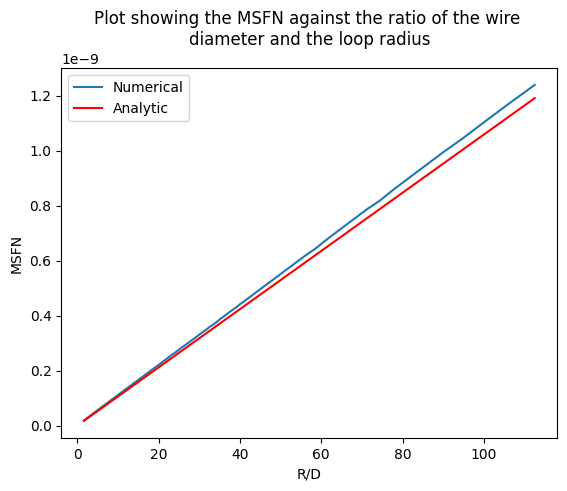
\includegraphics[width=\textwidth]{torusAVN}
        \caption{The meshed torus with the smallest loop radius and largest wire diameter}
        \label{fig:MSFNvRD}
    \end{subfigure}
    \hfill
    \begin{subfigure}[b]{0.48\textwidth}
        \centering
        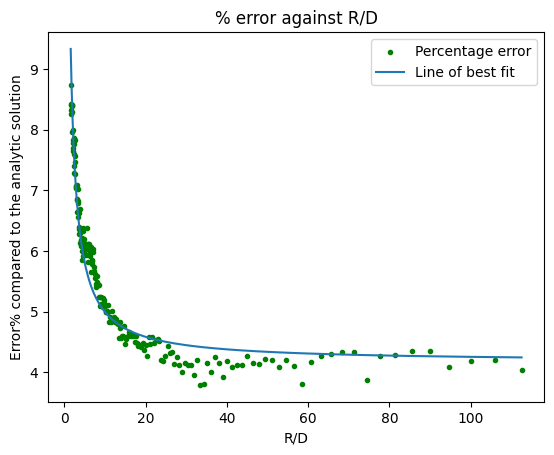
\includegraphics[width=\textwidth]{torusEVRD}
        \caption{The meshed torus with the largest loop radius and smallest wire diameter}
        \label{fig:evRD}
    \end{subfigure}
    \caption{A figure showing the two extremes of the parameter sweep for a torus. The images show the surface mesh as generated by GMSH.}
    \label{fig:resTorus}
\end{figure}
From figure \ref{fig:resTorus} it is clear to see that the relative percentage error compared to the analytic solution decreases as the ration of the loop radius to diameter increases. This behaviour can be attributed to the assumption: $R >> D$. The decrease in error clearly demonstrates that the noise extraction module works for this particular setup. In figure \ref{fig:MSFNvRD} the analytical and numerical results increase linearly with an increase in $\frac{R}{D}$ as expected.

\section{The mesh optimisation module}

\subsection{Test setup}
\subsection{Results}